\documentclass[a4paper,10pt]{report}

\topmargin -2cm
%\topskip0cm
%\footskip0cm
%\headsep0cm
\parindent0cm
\oddsidemargin -1cm
\evensidemargin -1cm
\headheight 2cm
\textheight 24cm
\textwidth 18cm

\author{Alexander M\"unn (4403061)}
\title{\"Ubung}

\usepackage{ucs}
\usepackage[utf8x]{inputenc}
\usepackage{german}
\usepackage{color}
\usepackage{url}
\usepackage{graphicx}
\usepackage{algorithmic}

\pagestyle{empty}
\usepackage{float}
\usepackage{makeidx}
\usepackage{amsmath}
\usepackage{amsfonts}
\usepackage{amssymb,euscript}
\usepackage{dsfont}
\usepackage{listings}
\usepackage{enumerate}
\newfont{\Fr}{eufm10}
\newfont{\Sc}{eusm10}
\newfont{\Bb}{msbm10}
\newcommand{\limin}{\lim_{n\rightarrow\infty}}
\newcommand{\limix}{\lim_{x\rightarrow\infty}}
\newcommand{\limun}{\lim_{n\rightarrow -\infty}}
\newcommand{\limux}{\lim_{n\rightarrow -\infty}}
\newcommand{\limx}{\lim_{x\rightarrow x_0}}
\newcommand{\limh}{\lim_{h\rightarrow 0}}
\newcommand{\defi}{\paragraph{Definition:}}
\newcommand{\bew}{\paragraph{Beweis:}}
\newcommand{\satz}{\paragraph{Satz:}}
\newcommand{\bsp}{\paragraph{Beispiel:}}
\newcommand{\lemma}{\paragraph{Lemma:}}
\newcommand{\N}{\mathds{N}}
\newcommand{\F}{\mathds{F}}
\newcommand{\Z}{\mathds{Z}}
\newcommand{\Q}{\mathds{Q}}
\newcommand{\R}{\mathds{R}}
\newcommand{\G}{\mathds{G}}
\newcommand{\C}{\mathds{C}}
\newcommand{\K}{\mathds{K}}
\newcommand{\A}{\mathds{A}}
\newcommand{\E}{\mathcal{E}}
\renewcommand{\P}{\mathcal{P}}
\newcommand{\sigA}{$\sigma$-Algebra }
\newcommand{\qed}{$\hfill\blacksquare$}
\newcommand{\arsinh}{\operatorname{arsinh} }
\newcommand{\arcosh}{\operatorname{arcosh} }
\newcommand{\gdw}{ $ \Leftrightarrow $ }
\newcommand{\tf}{ $ \Rightarrow $ }
\newcommand{\mgdw}{\Leftrightarrow}
\newcommand{\mtf}{\Rightarrow}
\newcommand{\Bild}{\text{Bild}}
\newcommand{\Kern}{\text{kern}}
\newcommand{\rg}{\text{rg}}
\newcommand{\deff}{\text{deff}}

\newcommand{\alphato}{\underset{\alpha}\to}
\newcommand{\betato}{\underset{\beta}\to}
\newcommand{\etato}{\underset{\eta}\to}
\newcommand{\ito}{\underset{i}\to}
\newcommand{\sto}{\underset{s}\to}
\newcommand{\kto}{\underset{k}\to}
\newcommand{\xto}{\underset{x}\to}

\usepackage{fancyhdr}
\pagestyle{fancy}
\lhead{Michael Borst\\ Alex Muenn}
\chead{"Ubungsblatt \nr\\\today}
\rhead{Computer Vision}



\newcommand{\nr}{1}

\begin{document}
\section*{Aufgabe 3 \& 4}

\begin{figure}[htpb]
\begin{center}
{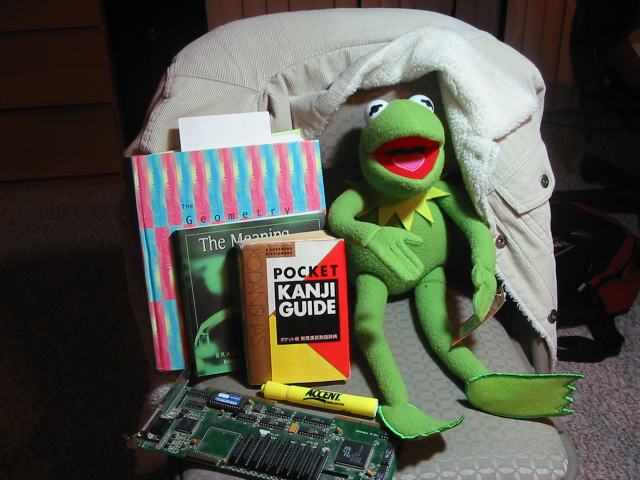
\includegraphics[width=0.25\textwidth]{samples/kermit001}}
\end{center}
\caption{Das Eingabebild für SIFT }
\label{fig:u02-picture}
\end{figure}

Folgende Funktion errechnet den (normierten) SIFT-Descriptor-Vektor.
Arbeitsschritte waren dabei Translation und Rotation des Koordinatensystems entsprechend dem Ort und der Orientierung des Descriptors, die Interpolation der Gradienten und dann die Aufteilung der Gradienten in die Bins der einzelnen Histogramme.

\lstset{language=matlab}
\begin{lstlisting}[caption={Berechnung des SIFT-Descriptor-Vektors}]
function SD = calculateSIFTDescriptor (Image, KeyPoint, rot, gridwidth, bsz, bins)
  # octave script to calculate sift descriptor for given keypoint

  [Dx, Dy] = gradient(Image, 0.5);

  step=2*pi/bins;


  SGx = zeros(gridwidth,gridwidth);
  SGy = SGx;
  # SIFT descriptor calculation needs its own coordinate system
  # compute x and y axis in image coordinate system
  #
  # +-----------> x
  # |
  # |  IMAGE
  # |  all angles are relative to top orientation (e.g. Vec(0 -1) has zero angle)
  # /
  # y
  #
  SDC_y = [-tan(rot*pi/180) 1];
  SDC_x = [1 tan(rot*pi/180)];
  SDC_x = SDC_x/norm(SDC_x);
  SDC_y = SDC_y/norm(SDC_y);
  # the origin of SIFT descriptor grid
  O = KeyPoint - (gridwidth/2-0.5)*(SDC_x+SDC_y);

  # fill grid with interpolated gradient information from origianl image gradients
  for y=1:gridwidth
    for x=1:gridwidth
      p = O + x*SDC_x + y*SDC_y;
      SGx(y,x) = gx = interp2(Dx,p(2), p(1));
      SGy(y,x) = gy = interp2(Dy,p(2), p(1));
      SG_magn(y,x) = norm([gx gy]);
    end
  end
  %-----------------------------------------------------------------------
  SG_theta = atan2(SGy, SGx) + pi;
  # unfortunatly SG_theta holds gradient angles in image space
  # we have to handle them relative to grids rotation
  SG_theta -= rot * pi/180;
  SG_theta = mod(SG_theta + 2*pi, 2*pi);
  # weight magnitude in the gaussian way
  g = gaussmatrix(gridwidth, gridwidth/2);
  SG_magn .*= g;

  SD = [];
  # 
  for b_y= 1:gridwidth/bsz
    for b_x = 1:gridwidth/bsz
      x=(b_x-1)*bsz+1;
      y=(b_y-1)*bsz+1;
      B_theta=SG_theta(x:x+bsz-1,y:y+bsz-1);
      B_magn=SG_magn(x:x+bsz-1,y:y+bsz-1);

      G_histo=zeros(1, bins);
      for row=1:bsz-1
        for col=1:bsz-1
          theta = B_theta(row,col);
          prevBin = floor(theta/step);
          nextBin = mod(prevBin+1,bins);
          prevBinDist = abs(prevBin*step-theta)/step;
          nextBinDist = 1-prevBinDist;
          mPrev = (1-prevBinDist)*B_magn(row,col);
          mNext = (1-nextBinDist)*B_magn(row,col);
          G_histo(uint8(prevBin+1)) += mPrev;
          G_histo(uint8(mNext+1))   += mNext;
        end
      end
      SD = [SD G_histo];
    end
  end
  # normalization of the feature vector
  SD = SD/norm(SD);
end
\end{lstlisting}



Folgende SIFT-Descriptoren wurden errechnet:

Aufgabe 3
\lstset{language=matlab}
\begin{lstlisting}[caption={Berechnung des SIFT-Descriptor-Vektors}]
SD3 =

 Columns 1 through 8:

   0.01570   0.00267   0.01191   0.00000   0.00000   0.00000   0.00463   0.00024

 Columns 9 through 16:

   0.08533   0.00131   0.01288   0.00000   0.00000   0.01873   0.02172   0.00000

 Columns 17 through 24:

   0.11271   0.00000   0.00000   0.00000   0.00000   0.01067   0.14542   0.01985

 Columns 25 through 32:

   0.01856   0.00000   0.00000   0.00000   0.00000   0.00000   0.00011   0.01001

 Columns 33 through 40:

   0.03069   0.01101   0.01930   0.00000   0.00000   0.00000   0.00000   0.00000

 Columns 41 through 48:

   0.11228   0.00000   0.00237   0.00000   0.00528   0.07531   0.00000   0.00000

 Columns 49 through 56:

   0.24943   0.00000   0.00000   0.00000   0.00000   0.03271   0.00978   0.00540

 Columns 57 through 64:

   0.01221   0.00000   0.00000   0.00000   0.00106   0.00256   0.00773   0.00092

 Columns 65 through 72:

   0.03768   0.01289   0.00000   0.00000   0.00000   0.00000   0.00000   0.02607

 Columns 73 through 80:

   0.16577   0.00080   0.02157   0.00000   0.00000   0.02691   0.01155   0.00000

 Columns 81 through 88:

   0.17192   0.00000   0.00000   0.00000   0.00000   0.04622   0.19050   0.00000

 Columns 89 through 96:

   0.01653   0.00000   0.00000   0.00000   0.00393   0.00131   0.00762   0.00000

 Columns 97 through 104:

   0.52367   0.00000   0.00000   0.00000   0.00000   0.00000   0.15472   0.60788

 Columns 105 through 112:

   0.18650   0.00364   0.02955   0.00000   0.00000   0.02787   0.00000   0.00000

 Columns 113 through 120:

   0.25423   0.00000   0.00000   0.00082   0.00114   0.03561   0.05874   0.00000

 Columns 121 through 128:

   0.01154   0.00000   0.00000   0.00231   0.00165   0.00408   0.00926   0.00000
\end{lstlisting}

Aufgabe 4
\lstset{language=matlab}
\begin{lstlisting}[caption={Berechnung des SIFT-Descriptor-Vektors}]
SD4 =

 Columns 1 through 8:

   0.11187   0.00302   0.00893   0.00000   0.00000   0.05915   0.00023   0.00000

 Columns 9 through 16:

   0.06989   0.01371   0.00000   0.00000   0.00000   0.01912   0.00215   0.00000

 Columns 17 through 24:

   0.22469   0.01862   0.00000   0.00000   0.00000   0.03664   0.05217   0.00000

 Columns 25 through 32:

   0.01839   0.00462   0.00341   0.00170   0.00154   0.00000   0.00000   0.00389

 Columns 33 through 40:

   0.02423   0.01786   0.00476   0.00000   0.00000   0.00000   0.00000   0.00000

 Columns 41 through 48:

   0.09776   0.00022   0.00000   0.00082   0.00209   0.12320   0.00000   0.00000

 Columns 49 through 56:

   0.24523   0.01525   0.00000   0.00000   0.00000   0.12810   0.00772   0.00000

 Columns 57 through 64:

   0.02319   0.00093   0.00000   0.00000   0.00245   0.00199   0.00176   0.00219

 Columns 65 through 72:

   0.06013   0.00000   0.00000   0.00000   0.00256   0.00254   0.00608   0.07701

 Columns 73 through 80:

   0.21764   0.11555   0.00000   0.00000   0.00000   0.09847   0.02491   0.00000

 Columns 81 through 88:

   0.31439   0.00182   0.00000   0.00498   0.00000   0.09208   0.00000   0.00000

 Columns 89 through 96:

   0.02466   0.00000   0.00043   0.00097   0.00592   0.00304   0.00000   0.00000

 Columns 97 through 104:

   0.37123   0.00000   0.00000   0.00589   0.00000   0.02458   0.66803   0.00000

 Columns 105 through 112:

   0.18625   0.07253   0.00000   0.00000   0.00223   0.06262   0.00000   0.00000

 Columns 113 through 120:

   0.04447   0.00000   0.01519   0.00000   0.00000   0.02161   0.00108   0.00000

 Columns 121 through 128:

   0.01243   0.00000   0.00264   0.00022   0.00624   0.00098   0.00141   0.00000
\end{lstlisting}

% \includegraphics[width=150mm]{<file.eps>}
\end{document}
